\documentclass[modern]{aastex631}
\bibliographystyle{aasjournal}


\usepackage{graphicx}
\usepackage[caption=false]{subfig}
\usepackage{amsmath}

% \usepackage{fontspec}
% \usepackage[T1]{fontenc}
% \usepackage{newtxsf}
% \setmainfont{Fira Sans Book}[Scale=1.0]

%\usepackage{booktabs}

\begin{document}
\shorttitle{Echelle Spectroscopy API}
\shortauthors{Gully-Santiago et al. }
\title{An Application Programming Interface for Echelle Spectroscopy}

\author{Michael Gully-Santiago}
\affiliation{University of Texas at Austin Department of Astronomy}

\author{TBD}
\affiliation{TBD}


\begin{abstract}

Modern \'echelle spectrographs produce information-rich echellograms that undergo standard reduction procedures to produce extracted 1D spectra, typically chunked into echelle orders.  The final post-processing steps for echelle orders are often left to the end-user scientists, since the order of opertations and algorithm choice may depend on the scientific application.  These steps---while uncontroversial and routine---act as a barrier to entry to newcomers, and act as a tax on scientific innovation since teams have to re-invent the wheel to overcome implementation complexity, before getting to the already inherently complex scientific enterprise.  Here we assemble a collection of standard post-processing algorithms into a single easy-to-use Application Programming Interface (API).  The open source permissively licensed Python 3 implementation \texttt{muler} lowers the barrier to entry and accelerates the investigation of astronomical spectra.  The framework currently supports data from the HPF, Keck NIRSPEC, and IGRINS spectrographs, and is extensible to others.

\end{abstract}

\keywords{High resolution spectroscopy (2096)}

\section{Introduction}\label{sec:intro}

Here is an annotated bibliography.

\begin{deluxetable}{chc}
  \tablecaption{Annotated bibliography for intro\label{table1}}
  \tablehead{
  \colhead{Reference} & \nocolhead{two} & \colhead{Key idea}
  }
  \startdata
  \citet{czekala15} & - & \texttt{Starfish} \\
  \citet{gullysantiago17} & - & Starfish modified for mixture models\\
  \citet{2019AJ....158..164B} & - & \texttt{wobble} \\
  Barentsen et al. & - & \texttt{lightkurve} \\
  \enddata
\end{deluxetable}


\section{Methodology: HPF}
\label{methods-details}
The HPF \texttt{Goldilocks} pipeline performs wavelength calibration and 1D spectral extraction, yielding the observed target spectrum confounded with the conspicuous instrumental blaze response, overall spectrally smooth system throughput efficiency, telluric absorption, and night sky emission lines.  We isolate the target astrophysical spectrum from the noisy, confounded spectrum through a series of post-processing steps described here.

There exists a correct order-of-operations to ``undo'' these confounding effects, since some terms appear additively and some multiplicatively.  We conduct these operations upon each of the $N=2048$ pixels $i$ on each of the $M=28$ spectral orders $m$ as vector operations, denoting the wavelength dependence $\boldsymbol{\lambda}_m = \begin{bmatrix}\lambda_{i=1} & \lambda_{i=2} & \cdots & \lambda_{i=N} \end{bmatrix}$ as a vector $\mathbf{f(\boldsymbol{\lambda})}_{m} = \begin{bmatrix}f_{i=1} & f_{i=2} & \cdots & f_{i=N} \end{bmatrix}$.  The entire HPF spectrum $\mathbf{F}$ of all orders concatenated end-to-end can be written as $\mathbf{F} = \begin{bmatrix} \mathbf{f}_{m=1} & \mathbf{f}_{m=2} & \cdots & \mathbf{f}_{m=M} \end{bmatrix}$.  The vector $F$ assembled in this way for HPF has $N\times M=57344$ pixels.  We also possess per-pixel uncertainty estimates $\boldsymbol{\sigma}_m$ for all pixels.  For notational simplicity we will stick to using $\mathbf{f(\boldsymbol{\lambda})}$ without the subscript $m$, with the rationale that most operations are performed per-order, so the order-level view of the spectrum becomes our predominant entry point to discussion.

Each HPF spectrum comes with two additional ancillary reference spectra obtained simultaneously with the target spectrum on the same 2D detector and extracted alongside in \texttt{Goldilocks}.  All observations contain a sky fiber spectrum, $\mathbf{f}_{\mathrm{sky}}$.  The other fiber is either an non-illuminated dark reference or else is directed to the Laser Frequency Comb (LFC).  We will simply denote this reference as $\mathbf{f}_{\mathrm{LFC}}$.  We distinguish the desired observed target star spectrum from these ancillary spectra through the addition of two subscripts: $\mathbf{f}_{\star,\mathrm{obs}}$.  The confounding process can be thought of as a black box function $g$:

\begin{equation}
\mathbf{f}_{\star, \mathrm{obs}} = g(\mathbf{f}_{\star}) + \boldsymbol{\epsilon_\sigma}
\end{equation}

where $\boldsymbol{\epsilon_\sigma}$ is a randomized realization of a noise vector with characteristic per-pixel uncertainty $\sigma_i$.  When written this way, it becomes clear that ``undoing'' or inverting the black-box function with some inverse operation $g^{-1}$ is inherently an inference procedure, since the noise instance is unknown.  For the purposes of this document we will assume our spectra possess such high signal-to-noise ratio that the uncertainty in these operations can be ignored when deriving best fit parameters.  In other words, we make no attempt to propagate uncertainty in associated with tuning parameters from those steps that involve obtaining a best fit value.

\subsection{Sky subtraction}
If the target fiber and sky fiber possessed exactly the same fiber throughputs and probed approximately the same air column, the first order of operations would be simply to subtract the observed reference sky flux from the target spectrum:

\begin{equation} \label{naive_sky_subtract}
\mathbf{f}_{\star, \mathrm{sky-free}} = \mathbf{f}_{\star, \mathrm{obs}} - \mathbf{f}_{\mathrm{sky}}
\end{equation}

In practice, the target fiber and sky fiber have different wavelength-dependent throughputs and probe columns of the Earth's atmosphere that are different enough to be perceived in the HPF spectrum at the few percent level.  A naive application of Equation \ref{naive_sky_subtract} therefore leaves behind skyline residuals that are inadequate for many scientific applications.  Instead we seek to develop an estimator $\mathbf{\hat{f}}_{\star, \mathrm{sky}}$ for the sky seen by the target fiber.  The simplest conceivable refinement to the naive sky model is merely to multiply by a scale factor, which may be either a scalar or vector:

\begin{eqnarray}
\mathbf{\hat{f}}_{\star, \mathrm{sky}} &=& \beta\cdot\mathbf{f}_{\mathrm{sky}}\label{refined_sky_subtract_scalar}
\\
\mathbf{\hat{f}}_{\star, \mathrm{sky}} &=& \boldsymbol{\beta}\odot\mathbf{f}_{\mathrm{sky}} \label{refined_sky_subtract_vector}
\end{eqnarray}

where $\odot$ symbolizes the element-wise product (\emph{aka} ``Hadamard product'') of a per-pixel scalar that physically means the fiber-integrated throughput depends on wavelength.  The $\beta$ term can be experimentally determined in two ways: either through flat-field calibration measurements ``Quartz FCU'', or through on-sky reverse-engineering.  First we determine $\beta$ from the flat-field calibration, by taking the ratio of the spectra taken between the target and sky fibers when illuminated by the same flat field lamp intensity pattern.  Figure \ref{fig:beta} shows $\boldsymbol{\beta}$ determined in this way.  We assembled 1903 flat field spectra acquired from January to mid-August 2021 and reduced with \texttt{Goldilocks}.  Figure \ref{fig:beta} shows the mean and 95\% region.  We see that the flux of the target spectrum routinely hovers around $4.5\%$ brighter than the sky spectrum.  In the absence of other information, we would expect a routine under-subtraction of the sky at this level.


\begin{figure*}[ht]
  \centering
  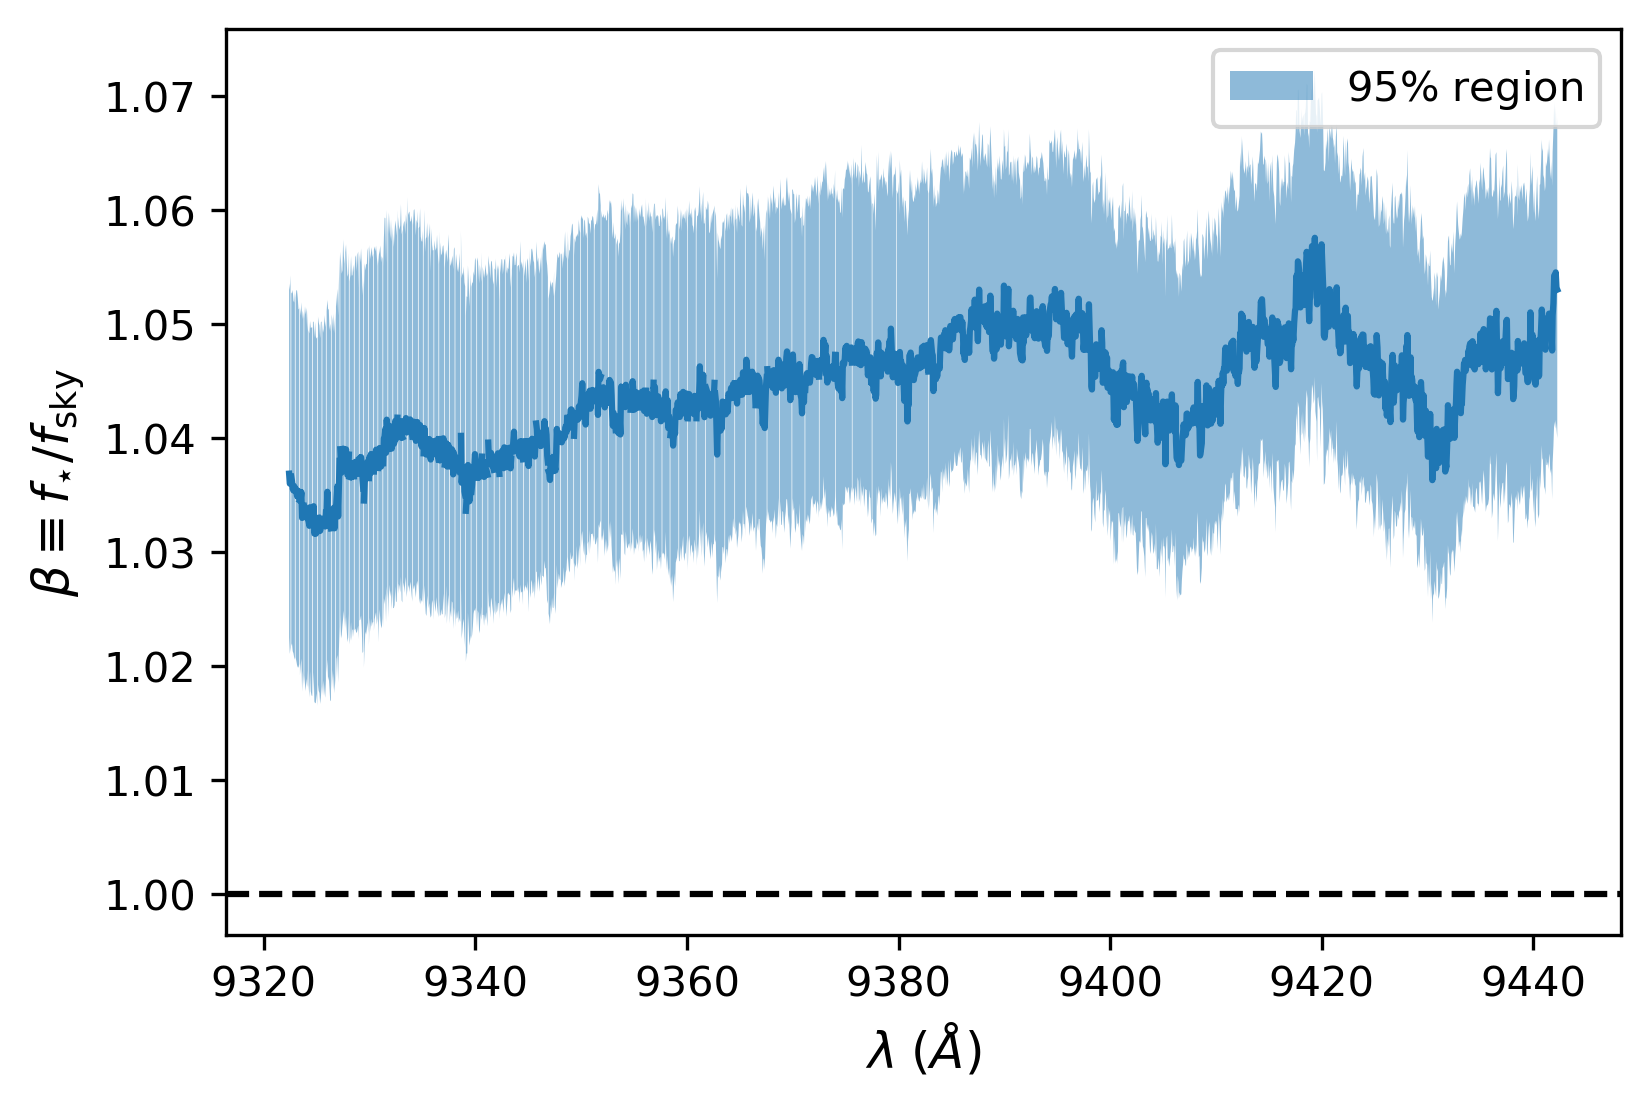
\includegraphics[width=0.55\textwidth]{figures/HPF_flat_field_demo.png}
\caption{Ratio of spectra from flat field illuminated target and sky fibers for HPF echelle order index $m=10$. \authorcomment1{The confidence region may be inaccurate, it would be wise to re-sample first.} }
\label{fig:beta}
\end{figure*}

The Quartz-illuminated calibration lamp does not contain differences in atmospheric column that exist in real astronomical observations.  We quantified the magnitude of this by retrieving 26 twilight flats obtained in 2021, and computing the ratio of the target fiber spectrum to sky fiber spectrum.  Typically we see that the target fiber perceives $8\%$ less flux than the sky fiber.  Figure \ref{fig:beta_twilight} of this ratio is shown for $m=25$ the spectral order possessing conspicuous $O_2$ telluric absorption bands.  You can see that the atmosphere is different enough between these two air columns to produce structure in the ratio.

With these data alone it is not clear the cause of the $8\%$ flux loss.  The root cause partly matters---is there something different about the way twilight flats are acquired compared to genuine science targets?  Why do we see different values for twilight flats and Quartz FCU flats (\emph{c.f.} Figure \ref{fig:beta})?  For now it is safe to say that the twilight flats are a better representation of a real science observation than the Quartz FCU: for whatever reason the target or ``science'' fiber sees about $8\%$ less flux than the sky fiber does.

Why is this scrutiny important?  If you blindly subtract the sky fiber from the science fiber, you will oversubtract individual spectral lines by $\sim8\%$, meaning you have reduced the line from $100\%$ to $-8\%$, a reduction of $12.5\times$.  Our goal is $0\%$ sky residuals, or as close to it as is feasible and below our signal-to-noise demands.  If we simply scale the sky fiber by $\beta=0.92$ using Equation \ref{refined_sky_subtract_scalar}, we may still not achieve $0\%$ residuals, but instead some value close to $1\%$, since the actual correction appears to vary from pixel-to-pixel, order-to-order, and from night-to-night at the $1\%$ level, the cause of which is unknown, but includes at least some uncertainty attributable to atmospheric path-length and small differences in Earth's atmospheric state towards the different sightlines.  Still a reduction from $8\%$ residual to $1\%$ residual is an $8\times$ improvement, and may already meet our specification.  Getting below $1\%$ residual would require some additional wavelength-based modeling of the twilight flats using Equation \ref{refined_sky_subtract_vector} and Figure \ref{fig:beta_twilight}.

The problem of sky subtraction is most acute for faint objects with long exposure times.  One such line resides close to the Helium 10830 line, so establishing the correct scale factor remains an important goal.

\begin{figure*}[ht]
  \centering
  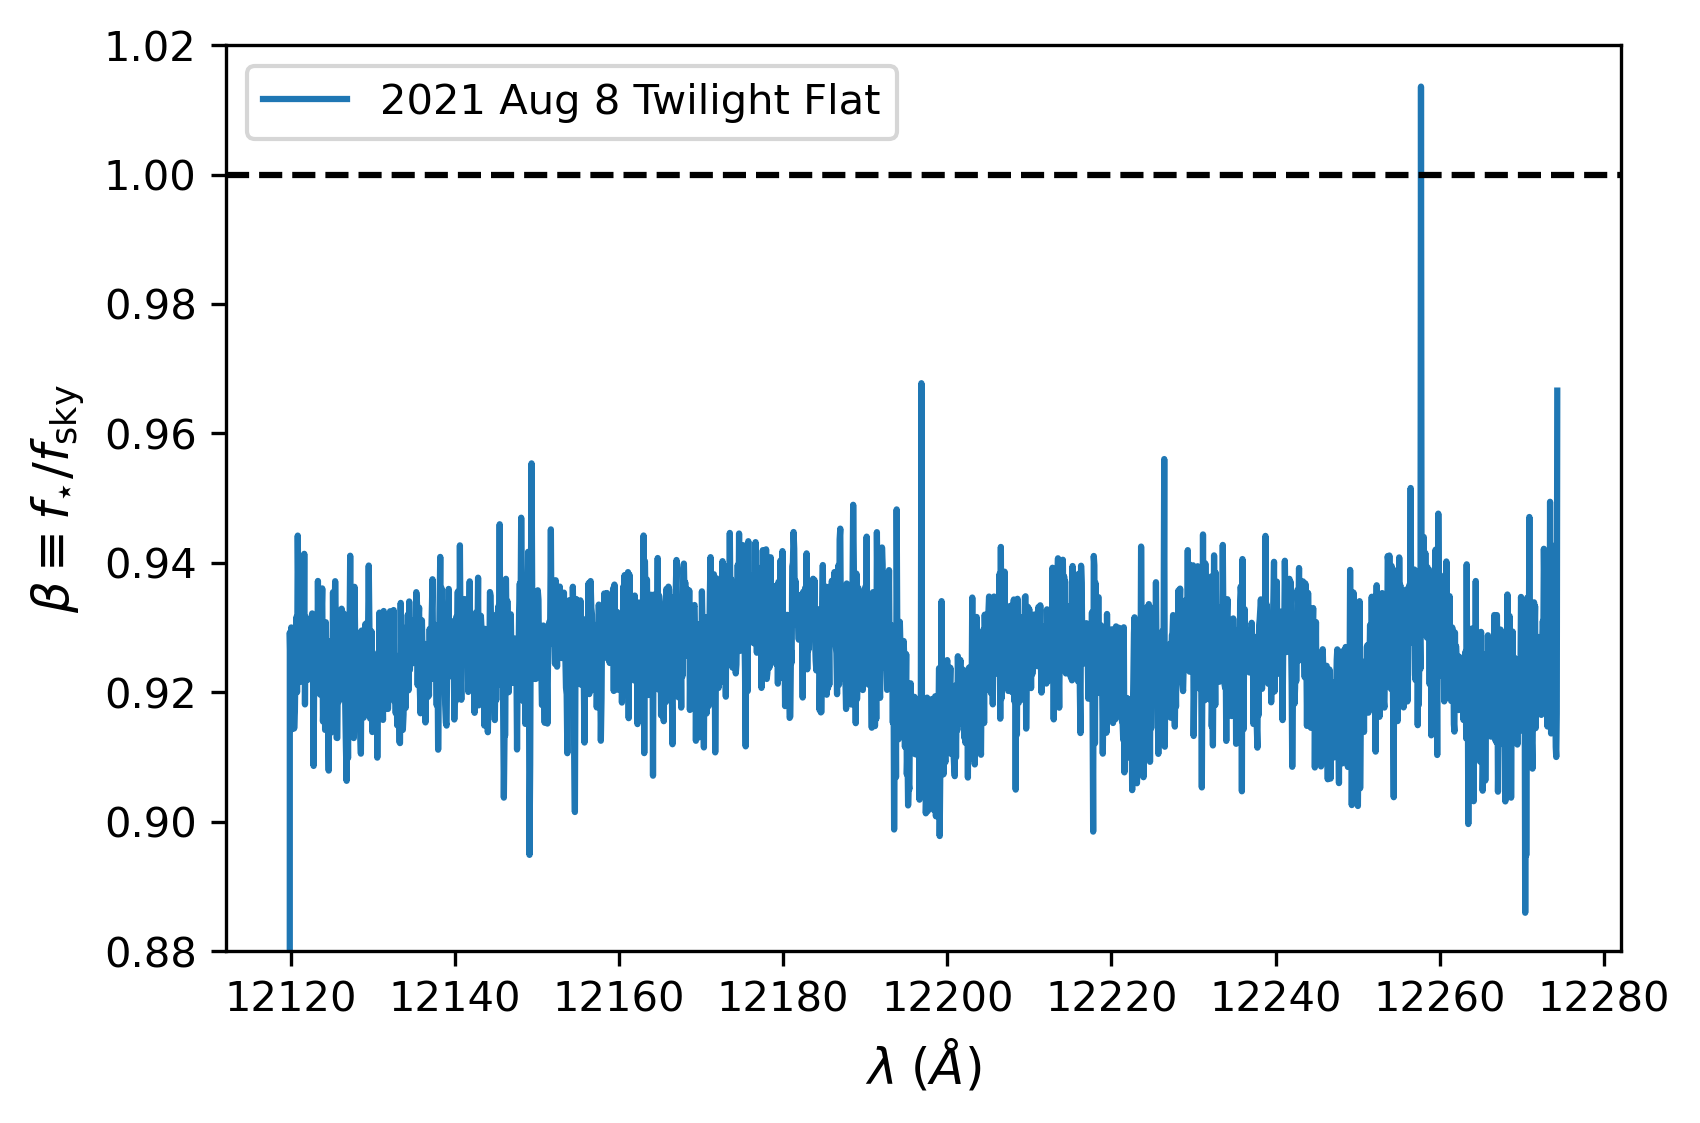
\includegraphics[width=0.55\textwidth]{figures/HPF_twilight_2021Aug8.png}
\caption{Ratio of spectra from \emph{twilight}-illuminated flat field target and sky fibers for HPF echelle order index $m=25$.  }
\label{fig:beta_twilight}
\end{figure*}

To summarize, we used both instrumental and on-sky calibration sources to estimate the differential throughput to the sky and target fibers.  We find that a wavelength dependent scale factor can conceivably improve sky subtraction.

\subsection{Deblazing and the instrumental response function}

We have previously seen instrumental throughput as a means of determining how much flux passes through different fibers.  Here we consider the spectral shape of the instrumental throughput.  The most conspicuous feature is the so called ``blaze function'' named after the characteristic inverted \emph{blaze envelope} that looks concave down: $^\frown$ imprinted by the \'echelle grating.  These shapes are highly stable, since they are an intrinsic property of the \'echelle grating and other instrumental properties, and the instrument is highly stabilized.

Here we assemble the same collection of 1903 Quartz FCU flat field spectra from 2021 to obtain a stock blaze correction.  The wavelength solution of the spectrograph can shift slightly, so we resampled all 1903 spectra onto a common 2048-pixel wavelength axis. We chose to normalize each spectrum in a way that would preserve the order-to-order variation.  For a single HPF spectrum we measure a global median flux value for all echelle orders, $m$.  We then divide the whole spectrum $\mathbf{F}$ by this value, leaving some orders with a mean value much greater than 1, and other orders with mean values much less than 1.  Finally we median combine all 1903 normalized spectra into a single $N\times M=57344$-pixel blaze spectrum.  The rationale for preserving the inter-order normalization is that it may convey some genuine information about the relative throughput among adjacent \'echelle orders.  The blackbody-like spectrum of the warm Quartz Lamp may imbue a spurious-albeit-smooth spectral tilt that we ignore.  Figure \ref{fig:blaze} shows the mean blaze shape.  The deviations from the mean are typically less than $2\%$, and exhibit smooth trends in time.

\begin{figure*}[ht]
  \centering
  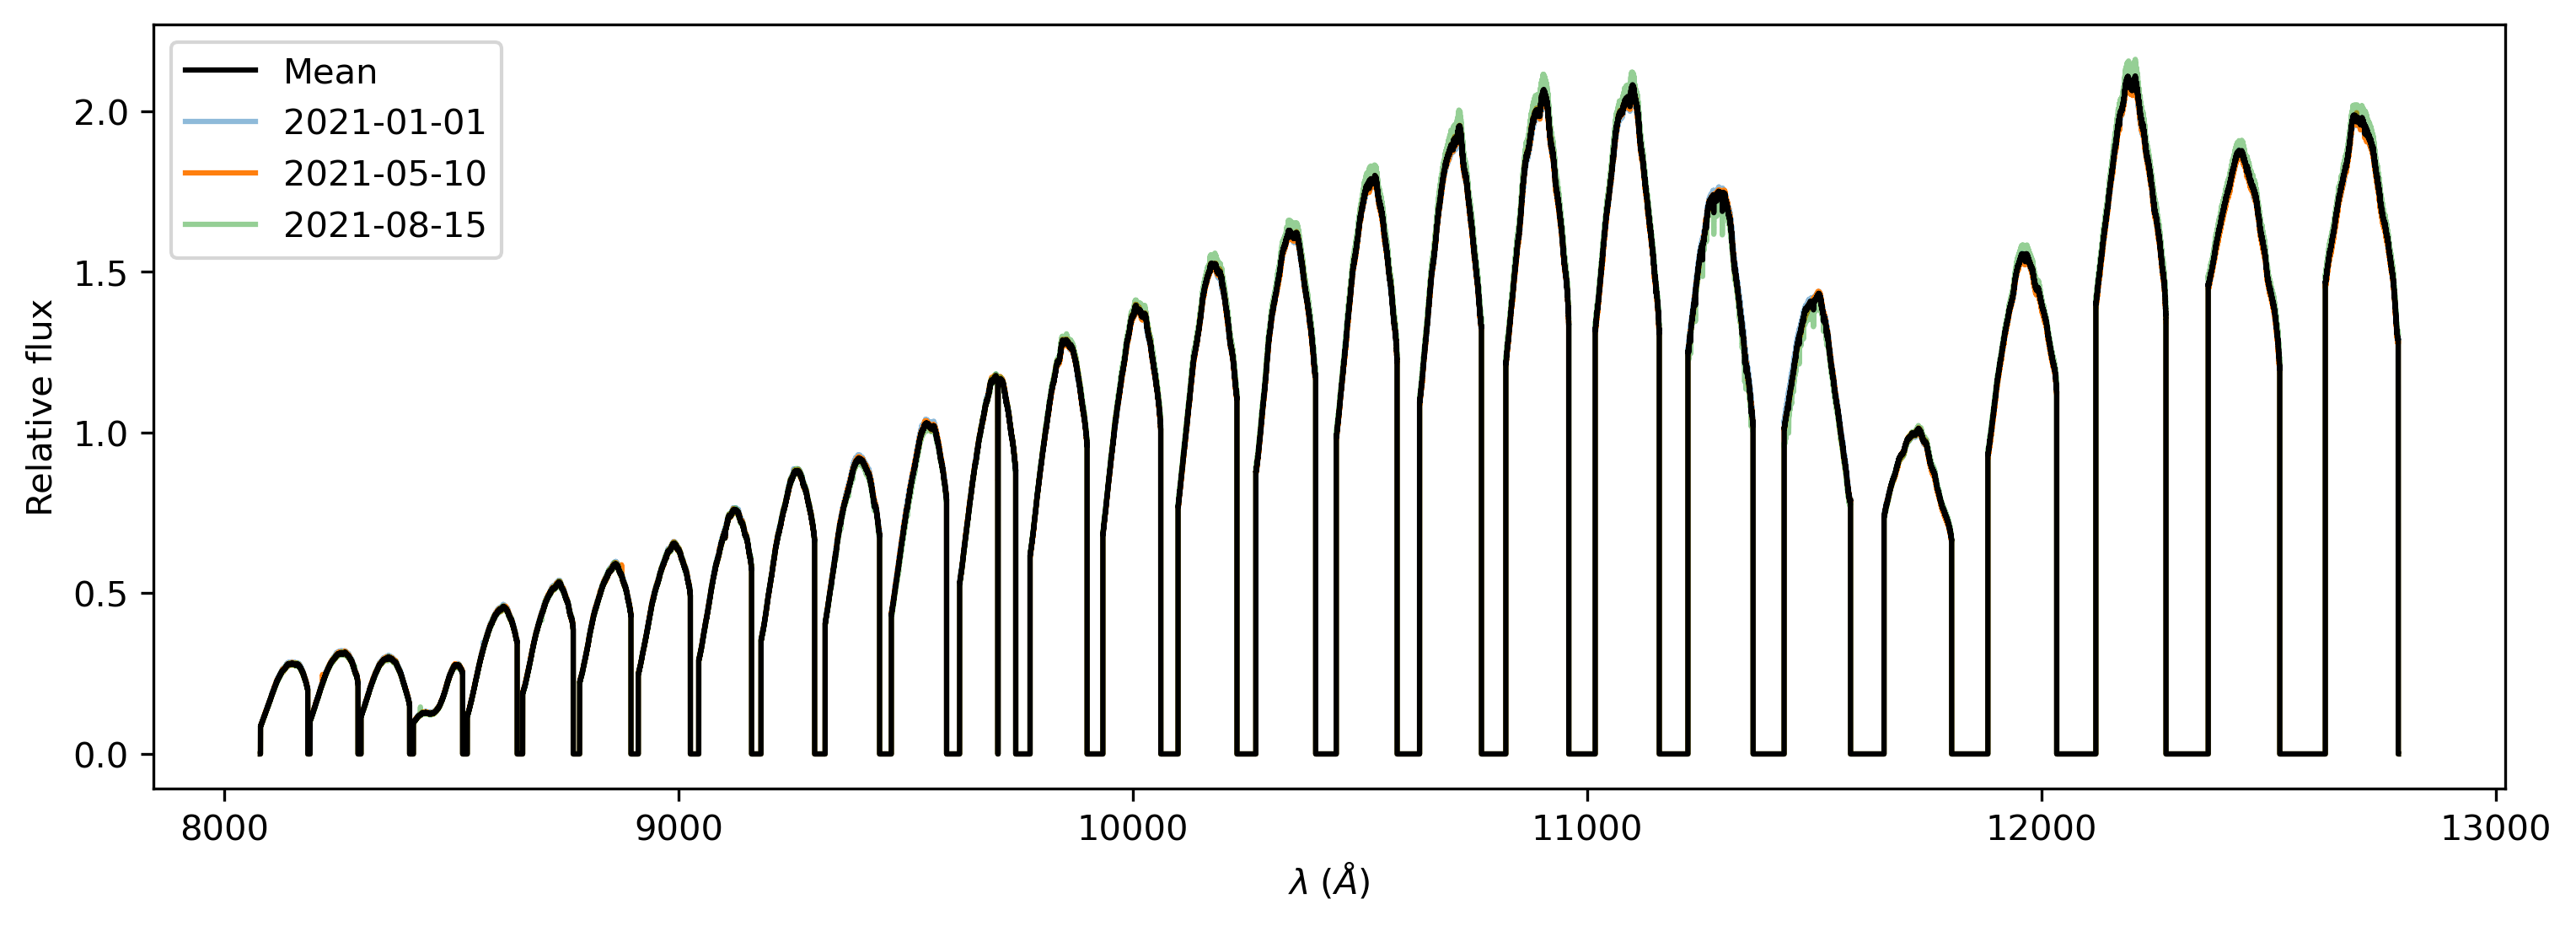
\includegraphics[width=0.95\textwidth]{figures/HPF_mean_blaze_function.png}
\caption{Mean blaze function for HPF, based on Quartz flat field calibration data.  Small month-to-month drifts imbue slight differences, examined in the next figure.}
\label{fig:blaze}
\end{figure*}

\begin{figure*}[ht]
  \centering
  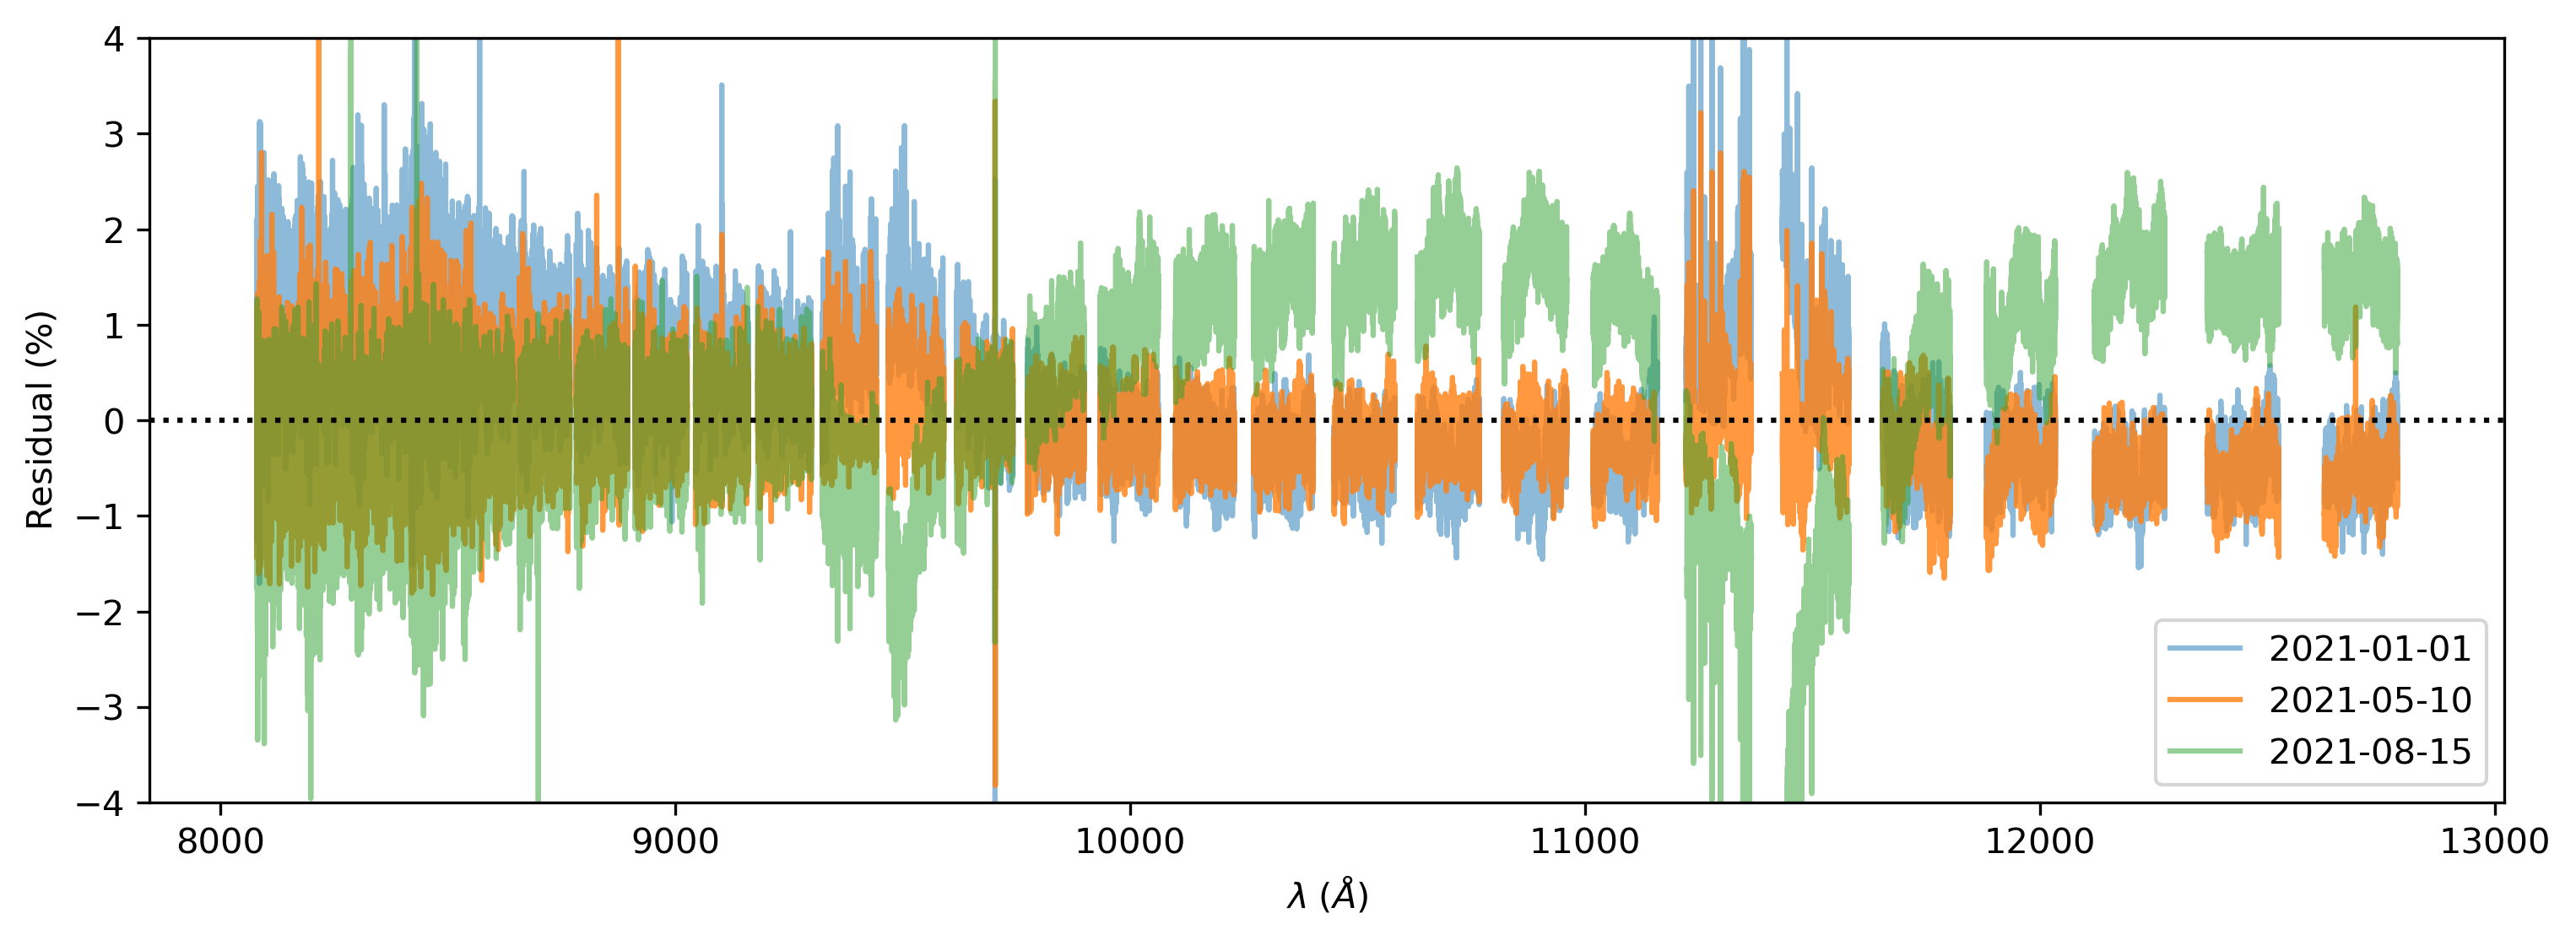
\includegraphics[width=0.95\textwidth]{figures/HPF_blaze_function_variation.png}
\caption{Blaze function residual spectra picked from 3 different nights separated by a few months.  The detailed shape of the blaze function drifts in time by a few percent.}
\label{fig:blaze_variation}
\end{figure*}

We divide all spectra (target star, standard star, and sky) by this mean blaze correction.  This step makes it much easier to view the typical spectral signals without the plunging signal at the spectrum edges.  Importantly blaze correction makes it easier to conduct spectral investigation on the A0V standard stars.  We can now mask telluric regions and then cross-correlate the spectrum with an A0V template to determine kinematic refinements to the A0V standard template.  The division yields the blaze free spectrum:

\begin{equation} \label{blaze_correction}
\mathbf{F}_{\mathrm{blaze-free}} = \mathbf{F}_{\mathrm{obs}}/ \mathbf{F}_{\mathrm{blaze}}
\end{equation}

We resample the mean blaze function to the observed wavelength grid to preserve the native observation grid.


\subsection{Standardizing telluric standards}
Most near-infrared spectral observing strategies include A0V standard star observations at some point during the course of observations, and typically at least once per night.  These typically A0V standard stars possess relatively few spectral features, with smooth undulations from Hydrogen lines.  The spectrum of these A0V stars is known extremely well due to their simplicity, and we therefore possess excellent theoretical estimators $\mathbf{\hat{f}}_{\mathrm{A0V,\;template}}$ that we will refer to as ``templates'', where scare quotes are intended to foreshadow the imperfect nature of these ostensibly static vectors.  After sky subtraction, all other instrumental signals are assumed to be \emph{multiplicative}.  You can therefore determine the wavelength-dependent instrumental response $\mathbf{r}_{\mathrm{inst}}$ by computing the ratio of sky-subtracted A0V spectrum to expected A0V template spectrum:

\begin{equation}
  \mathbf{r}_{\mathrm{inst}} = \frac{\mathbf{f}_{\mathrm{A0V,\;sky-free}}}{\mathbf{\hat{f}}_{\mathrm{A0V,\;template}}}
\end{equation}

Equipped with this instrumental response, we can hypothetically correct an observed, sky-subtracted science target spectrum with and element-wise multiplication:

\begin{equation}
  \mathbf{f}_{\mathrm{\star}} = \mathbf{f}_{\mathrm{\star,\;sky-free}} \oslash \mathbf{r}_{\mathrm{inst}}
\end{equation}

where $\oslash$ represents the element-wise division of vectors, that yields a vector of the same length $N$.  A few problems arise from this assumption, rank ordered below:

\begin{enumerate}
  \item The A0V standard star and target star $\star$ are acquired at different times and locations, and may therefore probe an atmospheric column with different total airmass, temperature-pressure profile, composition (\emph{i.e.} humidity), and cloud coverage.
  \item The A0V standard star template may not perfectly represent the observed standard star, and varies with BERV, intrinsic RV, and $v\sin{i}$
  \item The data generating process proceeds as a multiplication of target star spectrum and telluric absorption spectrum at native resolution, followed by convolution with the instrumental broadening kernel; convolution does not commute with multiplication.
  \item 
\end{enumerate}



\begin{acknowledgements}

The authors acknowledge the Texas Advanced Computing Center (TACC, \url{http://www.tacc.utexas.edu}) at The University of Texas at Austin for providing HPC resources that have contributed to the research results reported within this paper.
\end{acknowledgements}

\clearpage


\facilities{HET (HPF), IGRINS (Gemini South), NIRSPEC (Keck)}

\software{  pandas \citep{mckinney10, reback2020pandas},
  emcee \citep{foreman13},
  matplotlib \citep{hunter07},
  astroplan \citep{astroplan2018},
  astropy \citep{exoplanet:astropy13,exoplanet:astropy18},
  exoplanet \citep{exoplanet:exoplanet},
  numpy \citep{harris2020array},
  scipy \citep{jones01},
  ipython \citep{perez07},
  starfish \citep{czekala15},
  bokeh \citep{bokehcite},
  seaborn \citep{waskom14},
  pytorch \citep{NEURIPS2019_9015}} % No pytorch yet!


\bibliography{ms}

\end{document}
